\documentclass{llncs}

\usepackage{makeidx}
\usepackage{xspace}
\usepackage[dvips]{graphicx}
\usepackage{adjustbox}
\usepackage{graphicx}
\usepackage{blindtext}
\usepackage{algorithm}
\usepackage{cite}
\usepackage[noend]{algpseudocode}
\usepackage{multirow}
\usepackage{mathtools}
\usepackage{mathrsfs}
\usepackage{multicol}
\usepackage{enumitem}
\usepackage{extarrows}
\usepackage{caption}
\usepackage{subcaption}
\usepackage{amsmath, amsfonts, amssymb}
\usepackage{bbm}
\usepackage{stmaryrd}
\usepackage{mathtools}
\usepackage[mathscr]{eucal}
\usepackage{bm}
\usepackage{array}
\usepackage{url}
\usepackage{calc}
\usepackage{float}
\usepackage{latexsym}
\usepackage{multirow}
\usepackage{subcaption}
\usepackage{fmtcount}
\DeclareGraphicsExtensions{.eps,.jpg,.png,.pdf}
\usepackage[usenames, dvipsnames, table]{xcolor}
\usepackage{todonotes}
\usepackage[bookmarks,bookmarksdepth=2]{hyperref}
\hypersetup{colorlinks,linkcolor=black,urlcolor=blue}
\usepackage{multicol}
\usepackage{siunitx}
\usepackage{enumitem}
\usepackage{comment}
\usepackage{dashrule}
\usepackage{environ}
\usepackage{xargs}
\usepackage{hhline}
\usepackage{tikz}
\usepackage{circuitikz}
\usepackage{tikz-timing}[2009/12/09]
\usepackage{pgfplots}
\usetikzlibrary{shapes.geometric}
\usepackage{booktabs}
\usepackage{fixme}
\fxsetup{status=draft, nomargin, inline}
\fxusetheme{color}
\renewcommand{\algorithmicrequire}{\textbf{Input:}}
\renewcommand{\algorithmicensure}{\textbf{Output:}}

\newcommand\raisepunct[1]{\,\mathpunct{\raisebox{0.5ex}{#1}}}
\tikzset{latency/.style={path picture={ 
    \draw[black]
  (-.4, .1) -- (-0.1, 0.25) (-.4,.4) -- (-.1, 0.25);
  \draw[black]
  (-.4, .1) -- (-0.1, -0.05) (-.4,.-.2) -- (-.1, -0.05);
  }}}
  \tikzset{latencysbox/.style={path picture={ 
    \draw[black]
  (.3, -.5) -- (.45, -.2) (.45,-.2) -- (.6, -.5);
  }}}
\tikzset{mux 4by2/.style={muxdemux,
muxdemux def={Lh=4, NL=4, Rh=3,
NB=1, w=1, square pins=1}}}

\tikzset{mux 3by2/.style={muxdemux,
muxdemux def={Lh=4, NL=3, Rh=3,
NB=1, w=1, square pins=1}}}

\tikzset{mux 2by2/.style={muxdemux,
muxdemux def={Lh=3, NL=2, Rh=2,
NB=1, w=1, square pins=1}}}
\newcommand{\register}[1]{ node[rectangle, draw, minimum height = .75cm, minimum width = .75cm, name={#1}, bottomreg] {}}
\newcommand{\registerrot}[1]{ node[rectangle, draw, minimum height = .75cm, minimum width = .75cm, name={#1}, leftreg] {}}
\newcommand{\registerEn}[1]{ node[rectangle, draw, minimum height = .75cm, minimum width = .75cm, name={#1}, enable] {}}
\newcommand{\ro}[1]{ node[name={#1}, rectangle, rounded corners=3pt, minimum width=.5cm, minimum height=.8cm, draw, sparsam] {$\rho$}}
\newcommand{\rospa}[1]{ node[name={#1}, rectangle, fill = SPAgreen, rounded corners=3pt, minimum width=.5cm, minimum height=.8cm, draw, sparsam] {$\rho$}}
\newcommand{\rodpa}[1]{ node[name={#1}, fill = DPAblue, rectangle, rounded corners=3pt, minimum width=.5cm, minimum height=.8cm, draw, sparsam] {$\rho$}}
\newcommand{\tencdpa}[1]{ node[minimum size=1.25cm, fill = DPAblue, rounded corners=1ex, draw, name={#1}] {$\mathsf{\tilde{E}_{K, N}}$}}

\newcommand{\xor}[1]{ node[circle, inner sep=-1.3pt, name={#1}] {$\oplus$}}
\tikzset{bottomreg/.style={path picture={ 
  \draw[black]
(path picture bounding box.south west) -- (path picture bounding box.center) (path picture bounding box.south east) -- (path picture bounding box.center);
}}}
\tikzset{enable/.style={path picture={ 
  \node[] at (0,.25) {\footnotesize en};
    \draw[black]
(path picture bounding box.south west) -- (path picture bounding box.center) (path picture bounding box.south east) -- (path picture bounding box.center);
}}}
\tikzset{leftreg/.style={path picture={ 
  \draw[black]
(path picture bounding box.south west) -- (path picture bounding box.center) (path picture bounding box.north west) -- (path picture bounding box.center);
}}}
\newcommand{\xord}[1]{node [draw,circle,addition,minimum width=.4 cm, name = {#1}] {}}
\tikzset{addition/.style={path picture={ 
    \draw[black]
  (path picture bounding box.south) -- (path picture bounding box.north) (path picture bounding box.west) -- (path picture bounding box.east);
  }}}
  
\newcommand{\bitwidth}{\tikz{\draw[-] (-2pt,-2pt) -- (2pt, 2pt);}}

\tikzset{bitwidth/.style={above=-1pt, font=\tiny}}
\tikzset{bitwidthvert/.style={right = -1pt, font=\tiny}}
\usetikzlibrary{arrows, shapes.gates.logic.US, calc}
\tikzset{
  contact/.style={
    circle, 
    fill=black,
    minimum size=5pt, 
    inner sep=0pt,
    anchor=center,
  },
}
\newcommand{\andd}[1]{node [draw,circle,cross,minimum width=.4 cm, thick, name = {#1}] {}}
\tikzset{next/.style={->, >=latex}}
\tikzset{cross/.style={path picture={ 
    \draw[black]
  (path picture bounding box.south east) -- (path picture bounding box.north west) (path picture bounding box.south west) -- (path picture bounding box.north east);
  }}}
\tikzset{addition/.style={path picture={ 
    \draw[black]
  (path picture bounding box.south) -- (path picture bounding box.north) (path picture bounding box.west) -- (path picture bounding box.east);
  }}}
% color definition
\definecolor{SPAvgreen}{RGB}{0,154,23}
\definecolor{SPAgreen}{RGB}{127,255,0}
\definecolor{DPAblue}{RGB}{0,64,255}

\newcommand{\rate}{.5cm}
\newcommand{\perm}[1]{ node[rectangle, rounded corners=3pt, minimum width=.5cm, minimum height=1.8cm, draw, sparsam] {$\pi^{#1}$}}
\newcommand{\boxele}[1] {node [rectangle, rounded corners=3pt, minimum width=1.5cm, minimum height=1.2cm, draw, sparsam, thick, name = {#1}] {$\mathtt{#1}$}}
\newcommand{\permspa}[1]{ node[rectangle, fill = SPAgreen, rounded corners=3pt, minimum width=.5cm, minimum height=1.8cm, draw, sparsam] {$\pi^{#1}$}}
\newcommand{\permdpa}[1]{ node[rectangle, fill = DPAblue, rounded corners=3pt, minimum width=.5cm, minimum height=1.8cm, draw, sparsam] {$\pi^{#1}$}}
\newcommand{\permspav}[1]{ node[rectangle, fill = SPAvgreen, rounded corners=3pt, minimum width=.5cm, minimum height=1.8cm, draw, sparsam] {$\pi^{#1}$}}
\tikzset{sparsam/.style={inner sep=1pt}}
\newcommand{\xorspa}[1]{ node[circle, fill = SPAgreen, inner sep=-1.3pt, name={#1}] {$\oplus$}}
\newcommand{\xorspav}[1]{ node[circle, fill = SPAvgreen, inner sep=-1.3pt, name={#1}] {$\oplus$}}
\newcommand{\msg}{.7cm}
\newcommand{\minnext}{.4cm}
\newcommand{\phase}{1.7cm}
\newcommand{\xordpa}[1]{ node[circle, fill = DPAblue, inner sep=-1.3pt, name={#1}] {$\oplus$}}

\newcommand{\tbc}[1]{ node[minimum size=1.25cm,rounded corners=1ex, draw, name={#1}] {$\mathsf{\tilde{E}}$}}
\newcommand{\tbcdpa}[1]{ node[fill = DPAblue, minimum size=1.25cm,rounded corners=1ex, draw, name={#1}] {$\mathsf{\tilde{E}}$}}
\newcommand{\tbcspa}[1]{ node[fill = SPAgreen, minimum size=1.25cm,rounded corners=1ex, draw, name={#1}] {$\mathsf{\tilde{E}}$}}
\newcommand{\tbcspav}[1]{ node[fill = SPAvgreen, minimum size=1.25cm,rounded corners=1ex, draw, name={#1}] {$\mathsf{\tilde{E}}$}}

\newcommand{\skinnyll}{\ensuremath{S_{\mathrm{LL}}}\xspace}
\newcommand{\skinnyb}{\ensuremath{S_{\mathrm{B}}}\xspace}
\newcommand{\skinnys}{\ensuremath{S_{\mathrm{S}}}\xspace}
\newcommand{\asconp}{\ensuremath{\text{Ascon-p}}\xspace}

\newcommand{\randtake}{\overset{\$}{\gets}}
\renewcommand{\vec}[1]{\mathbf{#1}}
\newcommand{\sharing}[2][]{\vec{{#2}}^{#1}}
\newcommand{\gf}[1]{\mathbb{F}_{#1}}
\newcommand{\ft}{\gf{2}}
\newcommand{\reg}{\textsf{Reg}}
\newcommand{\func}[2]{#1\left(#2\right)}
\newcommand{\nShares}{d}
\newcommand{\algrule}[1][.2pt]{\par\vskip.5\baselineskip\hrule height #1\par\vskip.5\baselineskip}
\newcommand{\share}[3][]{\sharing[#1]{#2}_{#3}}

\newcommand{\algorithmautorefname}{Algorithm}
\def\sectionautorefname{Section} 
\def\subsectionautorefname{Section} 
\def\appendixautorefname{Appendix}


\begin{document} 
	
	\title{Side-Channel Analysis of Kyber's	Arithmetic Encodings: a Cautionary Note}
	%\author{Corentin Verhamme\inst{1} \and Ga\"{e}tan Cassiers\inst{1,2,3} \and Fran\c{c}ois-Xavier Standaert\inst{1}}
	%\institute{ICTEAM, Universit\'{e} catholique de Louvain, Louvain-la-Neuve, Belgium \and TU Graz, Graz, Austria \and Lamarr Security Research, Graz, Austria}
	%----------------------------------------------------------------
	\maketitle
	
	\begin{abstract}
		
	\end{abstract}
	
	
	\section{Introduction}
	
	It is not overstated to claim that the cryptography community is undergoing a major transition under the threat posed by quantum computing. Over the last few decades, building sufficiently large quantum computers has progressed from being physically impossible to merely an engineering hurdle. As a result, it puts many of the public-key cryptosystems currently in use at risk and, consequentially, compromises the confidentiality and integrity of digital communications. To prepare the information security systems to be able to resist quantum computing, in 2016, the USA National Institute of Standards and Technology (NIST) initialized a standardization process to promote quantum-resistant public-key cryptographic algorithms (also known as post-quantum cryptography, PQC). 
	
	After four rounds of evaluation, in 2022, NIST selected CRYSTALS-KYBER \cite{kyber} as the winner of Public-key Encryption and Key-establishment Algorithms. KYBER belongs to the lattice-based key encapsulation mechanism (KEM) family. Its hardness is based on the module learning-with-errors problem (M-LWE), which is conjectured to be hard to solve even by sufficiently large quantum computers. Despite the concrete mathematical security of the algorithmic designs, KYBER has been shown to be vulnerable under an implementation security perspective as more and more attacks from the Side-channel Attack (SCA) family have been proven to be effective. 
	
	SCAs were first studied in the late 1990s by Kocher \cite{kocher}, where it exploited the implementation execution time to reduce the computational cost of the key-recovering attack significantly. SCAs from then on have been spreading widely, and various  additional information, such as power consumption, electromagnetic emanation, photoemission, \dots, are utilized to thwart the implementations' security.
	
	Same as other lattice-based schemes, Kyber has been subjected to various SCAs. These attacks are diverse in terms of target procedure (e.g., Key Generation \cite{primas}, \cite{primas2}, \cite{liu}, Encapsulation \cite{menc1}, \cite{menc2}, \cite{menc3}, Decapsulation \cite{decaps1}, \cite{decaps2}, \cite{decaps3}, \dots), target operation within the procedure (e.g. Number Theoretic Transform (NTT), polynomial multiplication, Message Encode, KECCAK), attack vector (e.g. execution time, power consumption, Electromagnetic Emanation), etc. to name a few. Therefore, many studies have been dedicated to improving the side-channel resilience of Kyber's implementation by using countermeasures such as shuffling (e.g.,  \cite{shuffling}, \cite{menc1}), or masking (e.g.,  \cite{scr}, \cite{Kmask1}, \cite{Kmaskimp0}).
	
	
	
	Masking on Kyber differs from masking for former symmetric or asymmetric key schemes. The computations happen in power-of-two and prime-order groups. Thus, it requires both Boolean and arithmetic masking simultaneously, as well as their two-way conversion. Both masking schemes have been carefully studied and yielded very concrete, provable security levels \fxwarning{cite Provable sec for Boolean masking and arithmetic masking}. 
	
	Recently, arithmetic masking over prime-order group has been drawing attention, thanks to its natural noise amplification effect \cite{optimalmask}, \cite{primemask}. However, some constraints over these formal results prevent a direct generalization of its effectiveness on Kyber due to the special distribution of the secret. Therefore, in this note, we examine arithmetic masking, particularly for Kyber, to provide an atypical angle on its primary distinction from previously well-studied schemes and encourage further study on the subject.
	
	
	We first give several notions and notations needed for the note in Section \ref{sec:bg}. Next, an analysis of simulated data is carried out in Section \ref{sec:sim}. Finally, a quick evaluation proceeded on real measurements in Section \ref{sec:onm} to verify the former results' relevance.
	\section{Background}\label{sec:bg}
	Let us first lay out some notions regarding the arithmetic masking on Kyber.
	\subsection{Crystal-Kyber}
	\subsubsection{Polynomial Arithmetic}
	Kyber computations work on the polynomial ring $R_q = \mathbb{Z}_q[X]/(X^n + 1)$ where $q$ is a prime that allows efficient Number Theory Transformation, and $n$ is the size of message space. 
	A polynomial in such ring $\text{f}$ has the form as:
	\begin{equation}
		\text{f} = f_0 + f_1\cdot X^1 + \dots + f_{n-1}\cdot X^{n-1}
	\end{equation}
	where each coefficient $f_i$ lies in $\mathbb{Z}_q$.
	The secret $\mathbf{s}$ in Kyber is a vector of $k$ polynomials in $R^k_q$ such that each polynomial $\mathbf{s}[i] \in R_q$.
	
	\subsubsection{Centered binomial distribution}
	
	For the rest of this note, we use upper cases to denote random variables, lower cases to denote a realization of a random variable, and calligraphic letters to denote sets.
	
	A random variable $X$ we denote $X \overset{\$}{\leftarrow} \mathcal{X}$ where $X$ is uniform distributed over $\mathcal{X}$ and $X \leftarrow D$ when $X$ is chosen according to the distribution $D$.
	
	The noise (as well as secret) in Kyber is sampled from centered binomial distribution (CBD) $\beta_{\eta}$ for $\eta \in \mathbb{N}$, $s \leftarrow \beta_{\eta}$ and is computed as:
	\begin{align*}
		&(a_1, a_2, \dots, a_{\eta}, b_1, b_2, \dots, b_{\eta}) \overset{\$}{\leftarrow} \{0, 1\}^{2\eta}\\
		&s = \sum_{i=1}^{\eta}(a_i-b_i)
	\end{align*}
	
	The parameters set of Kyber for Round 3 of the NIST competition is summarized in the table below:\todo{Add spec table}
	Since this note focuses on polynomials encoding, we take $n, q, \eta$ value as in the table but keep $k=1$ for simplicity of the analysis.
	
	
	
	\subsubsection{Share Encoding}
	
	
	Masking is a popular countermeasure against DPA that aims to randomize the intermediate values processed by the device, thus making the side-channel leakage independent of the sensitive values. The core idea is to probabilistically split the sensitive variables into shares. The computations process on shares and only combine at the end to get the correct output. Masking generally works for most cryptographic schemes, is agnostic to the attack strategy, and guarantees a provable security.
	
	
	In a $d^{\text{th}}$-order masked implementation, each intermediate variable is concealed by $d + 1$ shares. The process of splitting a target value into $d+1$ \textit{random} values is called share encoding. The encoding representation determines the relations among shares and their target value, thus determines how the computations on shares are combined in the end. We extend the definition in \cite{Prouff13} to simplify the notations.
	\begin{definition}[$d$-share encoding]
		Let $\mathcal{X}$ be a set in a group $(\mathcal{G}, \ast)$ where $\ast$ is some group operation, and let $d$ be a positive integer. The $d$-share encoding of $x \in \mathcal{X}$ is a maps
		\begin{align*} 
			{Enc}^{\ast}_{d}: \mathcal{X} &\rightarrow \mathcal{G}^d:\\ 
			x &\mapsto ( x_1, \dots, x_d)
		\end{align*}
		such that $(x_i)_{i=1}^{d-1} \overset{\$}{\leftarrow} \mathcal{G}$ and $x = x_1 \ast x_2 \ast \dots \ast x_d$	
	\end{definition}
	Difference masking schemes have different encoding representations. For example, in symmetric schemes where the working group is $\mathbb{Z}_{256}$, for 2-share Boolean masking $\text{Enc}^{\oplus}_{2}(X) = (X_1, X_2)$ where $X_1 \overset{\$}{\leftarrow} \mathbb{Z}_{256},\ X_2 = X \oplus X_1$. In multiplicative masking, the encoding representation could be $\text{Enc}^{\otimes}_{2}(X) = (X_1, X_2)$ where $X_1 \overset{\$}{\leftarrow} \mathbb{Z}_{256} \text{ and } X_2 = X \otimes X_1 \text{ or } X_2 = X \otimes X_1^{-1}$.
	\todo{General masking scheme for KYBER}
	
	As mentioned earlier, the secret polynomial in Kyber can be expressed as a vector in $\mathbb{Z}_q$:
	$\text{s} = [s_0, s_1, \dots, s_n],\ s_i \leftarrow \beta_{\eta}$, all available masking schemes for polynomial computation of Kyber \fxwarning{citations} use additive arithmetic encoding, e.g.
	\begin{align*}
		Enc_2^{+}(s) &= (x_1, x_2)\\
		x_1 &\overset{\$}{\leftarrow} \mathbb{Z}_q^n\\
		x_2 &= s-x_1 \mod q
	\end{align*}
	For the rest of the note, we only study additive arithmetic encoding. Thus, to simplify the notation, we omit the operation specification of the encoding and keep $d$ subscript to specify the number of shares. 
	
	Furthermore, since the coefficients of $\text{s}$ are independent and the encoding acts on each coefficient independently, we only consider encoding for one coefficient (i.e., 1-D variable) instead of the entire polynomial (i.e., 256-D variable).
	
	Similar to multiplicative encoding in $\mathbb{Z}_{256}$, additive arithmetic encoding in $\mathbb{Z}_q$ can have different representations. To distinguish different representations, we use the superscript as an indicator, as an abuse of notation. Formally, for $\text{Enc}^{g}_{d}(X) = (X_1, X_2, \dots, X_d)$, 
	\begin{align*}
		&X_i \overset{\$}{\leftarrow}\mathcal{G}_q,\quad \text{for } i = 1,\dots, d-1, \\
		&X_d^g = g(X, X_1, \dots, X_{d-1}),
	\end{align*}
	where $g: \mathcal{X} \times \mathcal{G}^{d-1} \rightarrow \mathcal{G}$ dictates how the last share is computed, i.e. determines the encoding representation.
	Then in arithmetic encoding on $\mathbb{Z}_q$, we define two representations such as:
	\begin{align*}
		&\text{Enc}^{\text{sum}}_{d}(X) = (X_1, X_2, \dots, X_d)   ,  &  &\text{Enc}^{\text{diff}}_{d}(X) = (X_1, X_2, \dots, X_d) \\
		&X_d = X + \sum_{i =1}^{d-1}X_i   &  &X_d = X - \sum_{i =1}^{d-1}X_i ,
	\end{align*}
	where $X_i \overset{\$}{\leftarrow} \mathbb{Z}_q,\ \text{for } i \in \{1, \dots, d-1\}$.
	
	\subsection*{SCA Metrics and Distinguishers}
	We next recall some SCAs' relevant notions.
	\subsubsection*{Assumptions}
	First, let $X$ be the sensitive variable that is masked using the $d$-share encoding $\text{Enc}_d(X) = (X_1, X_2, \dots, X_d)$. The device carries computations on $(X_1, X_2, \dots, X_d)$ and produces corresponding leakage vector $\bm{L}(X) = (L_1, L_2, \dots, L_d)$.
	\paragraph{Independent Leakage and Independent Noise}
	The independence of the leakage allows us to re-write the leakage corresponding to each variable $X_i$ as $L_i = L(X_i)  = \delta_i(X_i) + B_i$, where $\delta_i$ is a deterministic function of $X_i$ and $B_i$ denotes the random noise. This assumption infers that the leakage from the device depends only on the data being processed.
	
	Noise Independency indicates the random noise $B_i$ in $L(X_i)$ is independent of the internal data $X_i$, (i.e. $L(X_i)  = \delta_i(X_i) + B$)
	\paragraph{Gaussian Leakage and Gaussian Noise}
	Gaussian leakage assumes that the distribution of the leakage $L_i$ given the variable $X_i$ follow is Gaussian, i.e., $(L_i|X_i=x) \leftarrow \mathcal{N}(\bm{m}_{i, x}, \bm{\Sigma}_{i, x})$, where $\bm{m}_{i, x}$ are expectation vectors and $\bm{\Sigma}_{i, x}$ are covariance matrices, both can be defined over high dimensional spaces.
	
	Gaussian Noise assumes that the distribution of the random noise $B$ follows a normal distribution with mean equal to zero and a standard deviation $\sigma$, i.e. $B \leftarrow \mathcal{N}(0, \sigma^2)$, or in other word, $(L_i|X_i=x) \leftarrow \mathcal{N}(\delta_i(x), \sigma^2)$.
	\subsubsection*{Signal-to-Noise Ratio}
	The signal-to-noise ratio (SNR) indicates the ratio between the signal and the noise component of measurement and is widely used in electrical engineering and signal processing. In this note, we use SNR as an initial tool to detect relevant points that seem to carry helpful information about the target value in the measurements (i.e., Point of Interest (PoI)).
	SNR of variable $X$ in leakage $\bm{L}$ is computed as
	\begin{equation*}
		\text{SNR} = \frac{Var_{X}[\mathbb{E}_{\bm{L}}[\bm{L}_x]]}{\mathbb{E}_{X}[Var_{\bm{L}}[\bm{L}_x]]}
	\end{equation*}
	\subsubsection*{Mutual Information and Perceived Information}
	\medspace
	Information-theoretic framework \fxwarning{IT citation} is a common tool to quantitatively analyze the worst-case security provided by a countermeasure. The mutual information (MI) measures the `amount of information  obtained about one random variable (e.g., the targeting variable $X$) by observing the other random variable (e.g., the leakage $\bm{L}$ corresponding to the computation on $X$) and is computed by:
	\begin{equation}\label{eq:mi}
		\text{MI}(X; \bm{L})  = \sum_{x\in \mathcal{X}} p(x)\cdot \log_2 p(x) + \sum_{x \in \mathcal{X}} p(x)\int_{\bm{l}\in \mathcal{L}^d}f(\bm{l}|x)\cdot \log_2 p(x|\bm{l}).
	\end{equation}
	The minuend is the self-entropy of $X$, $\text{H}(X)$ and the subtrahend is the conditional entropy of $X$ given $\bm{L}$, $\text{H}(X|\bm{L})$. 
	
	In Eq.\ref{eq:mi},  $p(x)$ is the probability mass function (PMD) of $X$ at the point $x$,  $f(\bm{l}|x)$ the Probability Density Function (PDF) of the leakage for a known value of $X=x$. and $p(x|\bm{l})$, followed the Bayes theorem, can be computed as
	\begin{equation}\label{eq:f2p}
		p(x|\bm{l}) = \frac{f(\bm{l}|x)p(x)}{\sum_{x'\in \mathcal{X}}f(\bm{l}|x')p(x')}.
	\end{equation}
	
	
	The MI value between $X$ and its leakage $\bm{L}$ directly links to the minimum number of measurements $N_a$ that an adversary must obtain in order to recover a specific value of $X$ \cite{mivsna}, \cite{mivsna2}:
	$$
	N_a \geq \frac{c(\text{sr}, |\mathcal{X}|)}{\text{MI}(\bm{L}; X)},
	$$
	where $c(\text{sr}, |\mathcal{X}|)$ is a small constant depends on the success rate $\text{sr}$ of the recovery attack, and size of the set $\mathcal{X}$.
	
	In practice, directly computing MI is a hard problem. One of the reasons is that the computational cost quickly becomes intractable as the dimension of $\bm{L}$ grows. In such a case, MI is usually estimated through a sampling process as follows:
	
	\begin{equation*}
		\widehat{\text{MI}}(X; \bm{L}) = \text{H}(X) + \sum_{x \in \mathcal{X}} p(x)\sum_{i=1}^{n_x}\frac{1}{n_x}\cdot \log_2 p(x|\bm{l}_{x, i}),
	\end{equation*}
	where $\bm{l}_{x, i}$ and $n_x$ are $i$th leakage trace and total number of traces corresponds to $X=x$, respectively. Estimation $\widehat{\text{MI}}$ converges to real MI as $n_x \rightarrow \infty$ \cite{lcert}.
	
	In addition, compute MI is not possible if $f(.|.)$, $p(.|.)$ are unknown priory. Then, these quantities are estimated through a sampling process as $\hat{f}(.|.)$ and $\hat{p}(.|.)$. The perceived information (PI) allows us to evaluate the quality of such estimations. Generally stated, PI quantifies the amount of information of $X$ that can be extracted from $\bm{L}$ using an estimated model $\hat{p}$ of $p$. The PI is theoretically defined as:
	\begin{equation*}
		\text{PI}(X; \bm{L}) = \text{H}(X) + \sum_{x \in \mathcal{X}} p(x)\int_{\bm{l} \in \mathcal{L}}f(\bm{l}|x)\cdot \log_2 \hat{p}(x|\bm{l}),
	\end{equation*}
	and is practically computed as a sampling process:
	\begin{equation}\label{eq:pi}
		\widehat{\text{PI}}(X; \bm{L}) = \text{H}(X) + \sum_{x \in \mathcal{X}} p(x)\sum_{i=1}^{n_x}\frac{1}{n_x}\cdot \log_2 \hat{p}(x|\bm{l}_{x, i})
	\end{equation}
	The sampling process that estimates $\widehat{\text{PI}}(X;  \bm{L})$ needs to be carried on a separate set that is used to estimate  $\hat{p}$ to ensure $\widehat{\text{PI}}$ is unbiased. It has been shown in \cite{lcert} that PI is upper bounded by MI, and the equality holds if the model $\hat{p}$ is perfect.
	
	It also has been pointed out in \cite{distinguishers} that PI provides a mean to compare different model $\hat{p}$s via their \textit{profiling complexity} and \textit{online attack complexity}. Loosely speaking, profiling complexity is the number of samples $N_p$ needed for an estimation $\hat{p}$ to reach a positive value, and the complexity of the best online attack can be performed with a model is the asymptotic PI value that can possibly reach by that model (i.e., $N_p$ is sufficiently high for the model to be optimal \fxwarning[]{wording}).
	
	We now detail several notations that involve the process of estimating the model $\hat{p}(x|\bm{l})$.
	
	
	\subsubsection*{Multivariate Gaussian Template}
	
	Multivariate Gaussian Template (MGT) aims to model the distribution $\hat{f}(\bm{l}|x)$ using the Gaussian Leakage assumption, i.e.
	\begin{equation}\label{eq:gmt}
		\displaystyle	\hat{f}(\bm{l}_i|x_i) = \frac{1}{\sqrt{(2\pi)^k\det \bar{\bm{\Sigma}}_{x}}}\exp\left(  -\frac{1}{2}(\bm{l}_i - \bar{\bm{m}}_{x})^T\bar{\bm{\Sigma}}_{x}^{-1} (\bm{l}_i - \bar{\bm{m}}_{x})\right) , 
	\end{equation}
	where $\bar{\bm{m}}_{x}$ and $ \bar{\bm{\Sigma}}_{x}$ are empirical means and covariance matrices correspond to value $x$ resulted from profiling data set. During the profiling phase, a template (i.e., mean and covariance matrix) has to be built for each value from the set of all possible values. 
	$\hat{p}(x|\bm{l})$ then can be estimated follows Eq.\ref{eg:f2p}.
	\subsubsection*{Linear Discriminant Analysis}\label{ssec:lda}
	Fisher's Linear Discriminant Analysis (LDA) is usually used in SCA as a pre-processing technique that aims to reduce the dimension of the leakage traces. LDA is known to be optimal in terms of minimizing the Bayes error for binary classification under normality and homoscedasticity assumptions \cite{LDAKojo}. LDA projects the original data to a subspace of lower dimension, the projection directions $\mathbf{w}$ is the solution of the maximization problem of the objective: $\frac{\mathbf{w}^T \mathbf{S}_B \mathbf{w}}{\mathbf{w}^T \mathbf{S}_W \mathbf{w}}$, where $\mathbf{S}_B, \mathbf{S}_W$ are respectively between-class scatter and within-class scatter matrices and is computed, respectively as:
	\begin{align*}
		\bm{S}_B &= \sum_{c=1}^{n_c}N(\bar{\mu}_c - \bar{\mu})(\bar{\mu}_c - \bar{\mu})^T,\\
		\bm{S}_W &=\sum_{c=1}^{n_c}\sum_{i=1}^N(\bm{l}^c_i - \bar{\bm{\mu}}_c) (\bm{l}^c_i - \bar{\bm{\mu}}_c)^T,
	\end{align*}
	where $\bar{\mathbf{\mu}}_c = \frac{1}{N_c}\sum_{i=1}^{N_c}\bm{l}^c_i$ is the mean of the traces corresponding to variable of class $c$, and,  $\bm{\mu} = \frac{1}{N}\sum_{c=1}^{n_c}\bar{\bm{\mu}}_c N_c$ is the total mean of all traces. Finding $\bm{w}$ is usually reduced to the problem of finding the eigenvectors of the matrix $\bm{S}_W^{-1}\bm{S}_B$.
	
	After LDA, the original data (e.g., $\bm{L}$) is transformed to lower dimension space (e.g., $\bm{L}_{lda} = \bm{L} \bm{w}$) since the number of classes is usually smaller than the original dimension. However, it has been shown in\fxwarning{LDA in SCA citations} that only a few of the eigenvectors that correspond to the highest eigenvalues are sufficient. The dimension after projection also affects the performance of LDA. 
	
	\todo{MGT after LDA}
	%As mentioned before, LDA is based on the homoscedasticity assumption, i.e., the same covariance matrix for all classes. Hence, if
	After LDA projection, MGT can be applied to the projected data where the covariance matrices of all classes are pooled into one. Then, the probability in Eq.\ref{eq:gmt} has the form:
	\begin{equation}\label{eq:gmt}
		\displaystyle	\hat{f}(\bm{l}_i|x_i) = \frac{1}{\sqrt{(2\pi)^k\det \bar{\bm{\Sigma}}_{x}}}\exp\left(  -\frac{1}{2}(\bm{l}_i - \bar{\bm{m}}_{x})^T\bar{\bm{\Sigma}}_{x}^{-1} (\bm{l}_i - \bar{\bm{m}}_{x})\right) , 
	\end{equation}
	where $\bar{\mathbf{\mu}}_c $ are computed on projected traces, and the pooled covariance matrix $\bm{\Sigma}$ is computed as:
	$$\bm{\Sigma} = \frac{1}{N}\sum_{x \in \mathcal{X}} n_x \bm{\Sigma}_x$$
	\subsubsection*{Multi-Layer Perceptron} 
	Multi-Layer Perceptron (MLP) acts as an efficient tool for supervised classification problem \fxwarning{few citations} and is extensively used in SCA. An MLP is composed of several different  trainable layers (i.e. ). In its simplest form, MLP usually has a few pairs of \textit{linear layer} directly followed by a \textit{non-linear activation function}, sequentially stacked up, and then finally outputs a discriminative model using a \textit{sofmax} layer. 
	
	During the training phase, the parameters of the layers are gradually changed in the direction that optimizes an objective. We set the objective to be minimizing the Negative Logarithm Likelihood Loss, since it was shown in \cite{DNN} to be relevant to profiled SCA.
	
	Using NLL loss as the objective, we can also use the validation loss of the network to estimate the PI value of the training model $p$. Thus, we apply the Early Stopping technique, where the criteria is the minimal validation loss (in other words, maximal validation PI). 
	
	MLP can be used in our analysis as a general (no specific assumption required) and straightforward (input the leakage traces directly) model. Therefore, it is used to estimate models on sensitive variables as well as on different shares of the target one.
	\subsection*{Soft-Analytical Side-channel Attack}
	Soft-analytical side-channel Attack (SASCA) was first introduced in \cite{sasca} and has been extensively used in recent studies (\cite{lcert}, \cite{mshares}, \cite{primemask}, \dots). The Belief-Propagation (BP) algorithm at the core of the method allows many time samples (corresponding to many intermediate variables) in the leakages to be exploited simultaneously while keeping the computational cost reasonable enough. \fxnote[]{wording}
	
	We also apply SASCA in this note to extend our study to widen the scenario, similarly in \cite{primemask} and \cite{mshares}, with some changes to fit our problem.
	
	Recall that the PDF $f(\bm{l}|x)$ in $d$-share encoding implementation can be rewritten as the convolution of each share leakage component. Precisely, if $\text{Enc}_d(S) = (X_1, \dots, X_d)$ then 
	\begin{equation}
		f(\bm{l}|s) = \sum_{\substack{x_1,\\\dots, \\x_{d-1} \in \mathbb{Z}_Q}}f(\bm{l}|s, x_1, \dots, x_{d-1})\cdot p(x_1, \dots, x_{d-1}),
	\end{equation}
	where $X_i \overset{\$}{\leftarrow} \mathbb{Z}_Q$, independently, for $i\in {1, \dots, d-1}$. If we consider the independent leakage assumption, we have
	\begin{equation}
		f(\bm{l}|x) = \sum_{\substack{x_1,\\\dots, \\x_{d-1} \in  \mathbb{Z}_Q}}\prod_{i=1}^{d}f(l_i|x_i)\cdot \prod_{i=1}^{d-1}p(x_i).
	\end{equation}
	Plug this expression into Eq.\ref{eq:f2p} we have
	\begin{equation}
		p\left( s|\bm{l}\right)  = \sum_{\substack{x_1,\\\dots, \\x_{d-1} \in \mathbb{Z}_Q}} \prod_{i=1}^{d} p\left( x_i|l_i\right) \frac{p(s)}{p(x_d)},
	\end{equation}
	where $x_d = s \pm \sum_{i=1}^d x_i$.
	
	When $p(x_i|li)$ are known (e.g. results from a model or through knowing $f(l_i|x_i)$ in simulation), we instantiate $r^0_{ii} = f_i(x_i)$ where $f_i(x_i) = p(x_i|l_i)$ and $r^0_{ss} = p(s)/Q$, run BP for two steps, we can read out the message at note $S$ as:
	\begin{equation}
		Z_s(s) = \frac{p(s)}{Q} \cdot\sum_{\substack{x_i\in  \mathbb{Z}_Q \\ \sum x_i = s}} \prod_{i=1}^{d} p\left( x_i|l_i\right), 
	\end{equation} 
	and obtain the expected value.
	
	
	\section{Simulated analysis} \label{sec:sim}
	We first try to investigate the difference between representations on simulated data. Same reason as several similar studies \cite{distinguishers}, \cite{primemask} on the related subject, this allows us to inspect them in a wider range of scenarios (from very low noise to high noise levels, from a small number of shares to sufficiently high ones).
	
	Recall that we only focus on masking the prime-field arithmetic operations, and especially on the sensitive variables that lie in a small range of the field (i.e., results from CBD sampling). Let the sensitive variable is $S$, then the sensitive set $\mathcal{S}$ equals to $\left\lbrace 0, 1, 2, -1, -2 \right\rbrace $ corresponding to the probability $P_{\mathcal{S}} = [ 0.375,  0.25,   0.0625, 0.25,   0.0625]$. 
	
	The encoding under investigations are $\text{Enc}^{\text{sum}}_{d}$ and $\text{Enc}^{\text{diff}}_{d}$ where the shares $X_i$ are drawn at random from $\mathbb{Z}_Q$ for $i \in \left\lbrace 1, \dots, d-1\right\rbrace $, where $Q$ is 3329 as proposed by KYBER's authors. The last share $X_d$ is computed differently for each representation, $X_d^{\text{sum}} = S + \sum_{i = 1}^{d-1} X_i$ while $X_d^{\text{sum}} = S - \sum_{i = 1}^{d-1} X_i$.
	
	The leakage vector corresponding to the processing of $S$ is $\bm{L}$ is simulated as the concatenation of the leakage corresponding to the individual shares i.e., $\bm{L} = \left[ L_1, \dots, L_d \right] $. We consider the Hamming Weight (HW) model, i.e., $\delta(X_i) = \text{HW}(X_i)$, since it is the most used in theoretical analysis \cite{2dpa} and was proven to be relevant to real-life setups for CMOS devices\fxwarning[]{citations}. We also assume Gaussian Noise, i.e. $L_i = \text{HW}(X_i) + b_i$ where $b_i \leftarrow \mathcal{N}(0, \sigma^2)$. 
	
	To recap, the leakage corresponding to sensitive variable $S$, which is encoded as $(X_1, X_2, \dots, X_d)$, is a vector $\bm{L} = \left[ \text{HW}(X_1) + b_1, \text{HW}(X_2) + b_2, \dots, \text{HW}(X_d) + b_d \right] $, where $b_i \leftarrow \mathcal{N}(0, \sigma^2) $. Precisely, the probability of the share leakage gives its value in the form:
	\begin{equation}\label{eq:gl}
		f(l_i|x_i) = \frac{1}{\sigma\sqrt{2\pi}} e^{ -\frac{1}{2}\left( \frac{\text{HW}(x_i)}{\sigma}\right) ^2 }.
	\end{equation}
	
	Accordingly, SNR can be computed as a function of the noise $\sigma$, note that $\mathbb{Z}_Q \subset \mathbb{Z}_{2^{11}}$:
	$$\text{SNR} \approx \frac{2.76}{\sigma}$$
	
	Ultimately, we use $d$ (i.e., the number of shares) and $\sigma$ (i.e., the noise level of the implementation) as the parameters of the analysis since they determine the security level of masking countermeasure \fxwarning[]{citations}.
	
	
	\subsection{2-share leakage distributions}
	
	Theoretically, second-order DPA is possible if the joint probability distributions are different for different sensitive values $s$ (i.e., key-dependent). This has been clearly shown to be relevant in the context of 8-bit Boolean masking, where each Hamming Weight value of 9 possible values produces one distinct leakage distribution (Figures 11, 12, 13 in \cite{2dpa}).
	
	Since the computations now moved from binary field to prime field, encoding operation moves from exclusive-or (XOR) to arithmetic ones, the distinctiveness of these distributions becomes 
	less obvious. For example, the distributions for $\text{Enc}^{\text{sum}}_{d}$ with uniform $S$ over $\mathbb{Z}_5$ is shown in Fig.\ref{fig:dist5_sum}, we use histogram to estimate such distributions. For the same $\text{HW}=1$, $s=1, 2, 4$ have three distinct shapes. 
	\begin{figure}
		\vspace*{-0.0cm}
		\hspace*{0.0cm}\centering 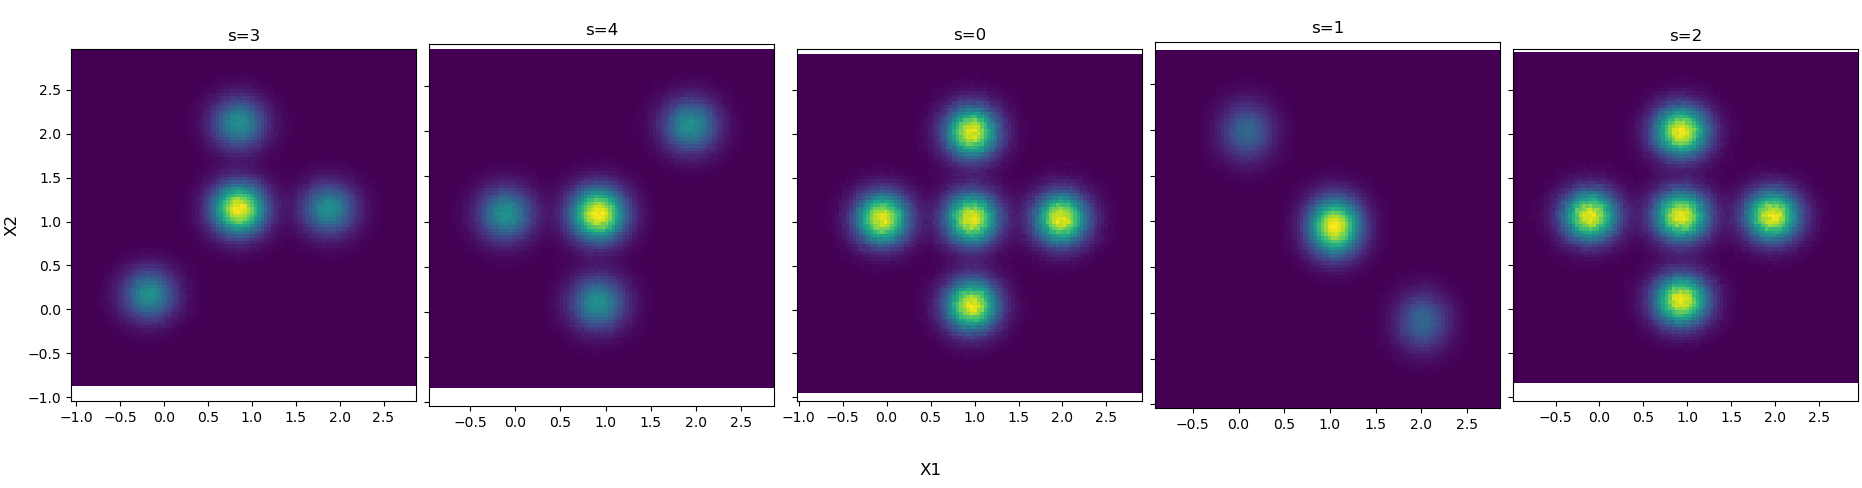
\includegraphics[width=12.0cm]{figures/5_dist_sum.png}
		\vspace*{0.3cm}
		\caption{2-share leakage distributions over $\mathbb{Z}_5$, uniform sensitive variable.}\label{fig:dist5_sum}\vspace*{-0.0cm}
	\end{figure}
	
	Intuitively, the XOR operation acts independently for each bit, leading to certain \fxnote[]{wording} relations among operands' HWs (e.g., $\text{HW}(X\oplus Y) = \text{HW}(X) + \text{HW}(Y) - 2\cdot\text{HW}(X\times Y)$), hence, produces well-separate distribution shapes for each value. The arithmetic operations (e.g., addition, subtraction, modulo) let results from lower-order bits affect higher-order bits through the carry (or borrow) bits, leading to more unclear connections. In addition, because it is frequently applied at the end, the binary representation of the moduli has a significant impact on the variety of the distribution shapes.
	\todo{Add more info on dist of diff prime in A?}
	
	If $S$ is uniform over $\mathbb{Z}_Q$, there should not be much difference between representations. For example, in Fig.\ref{fig:dist5}, \ref{fig:dist11}, we can see even though they look different in shapes, generally, they have the same number of shapes.
	
	However, when we take the small support of $S$ into account, the dissimilarity of these distributions generated by different encoding representations emerges clearly. In  Fig.\ref{fig:dist}, there certainly is a significant difference between the two representations. It is reasonable to question the gap in the amount of information about sensitive variable $S$ given these two sets of distributions.
	\begin{figure}
		\centering 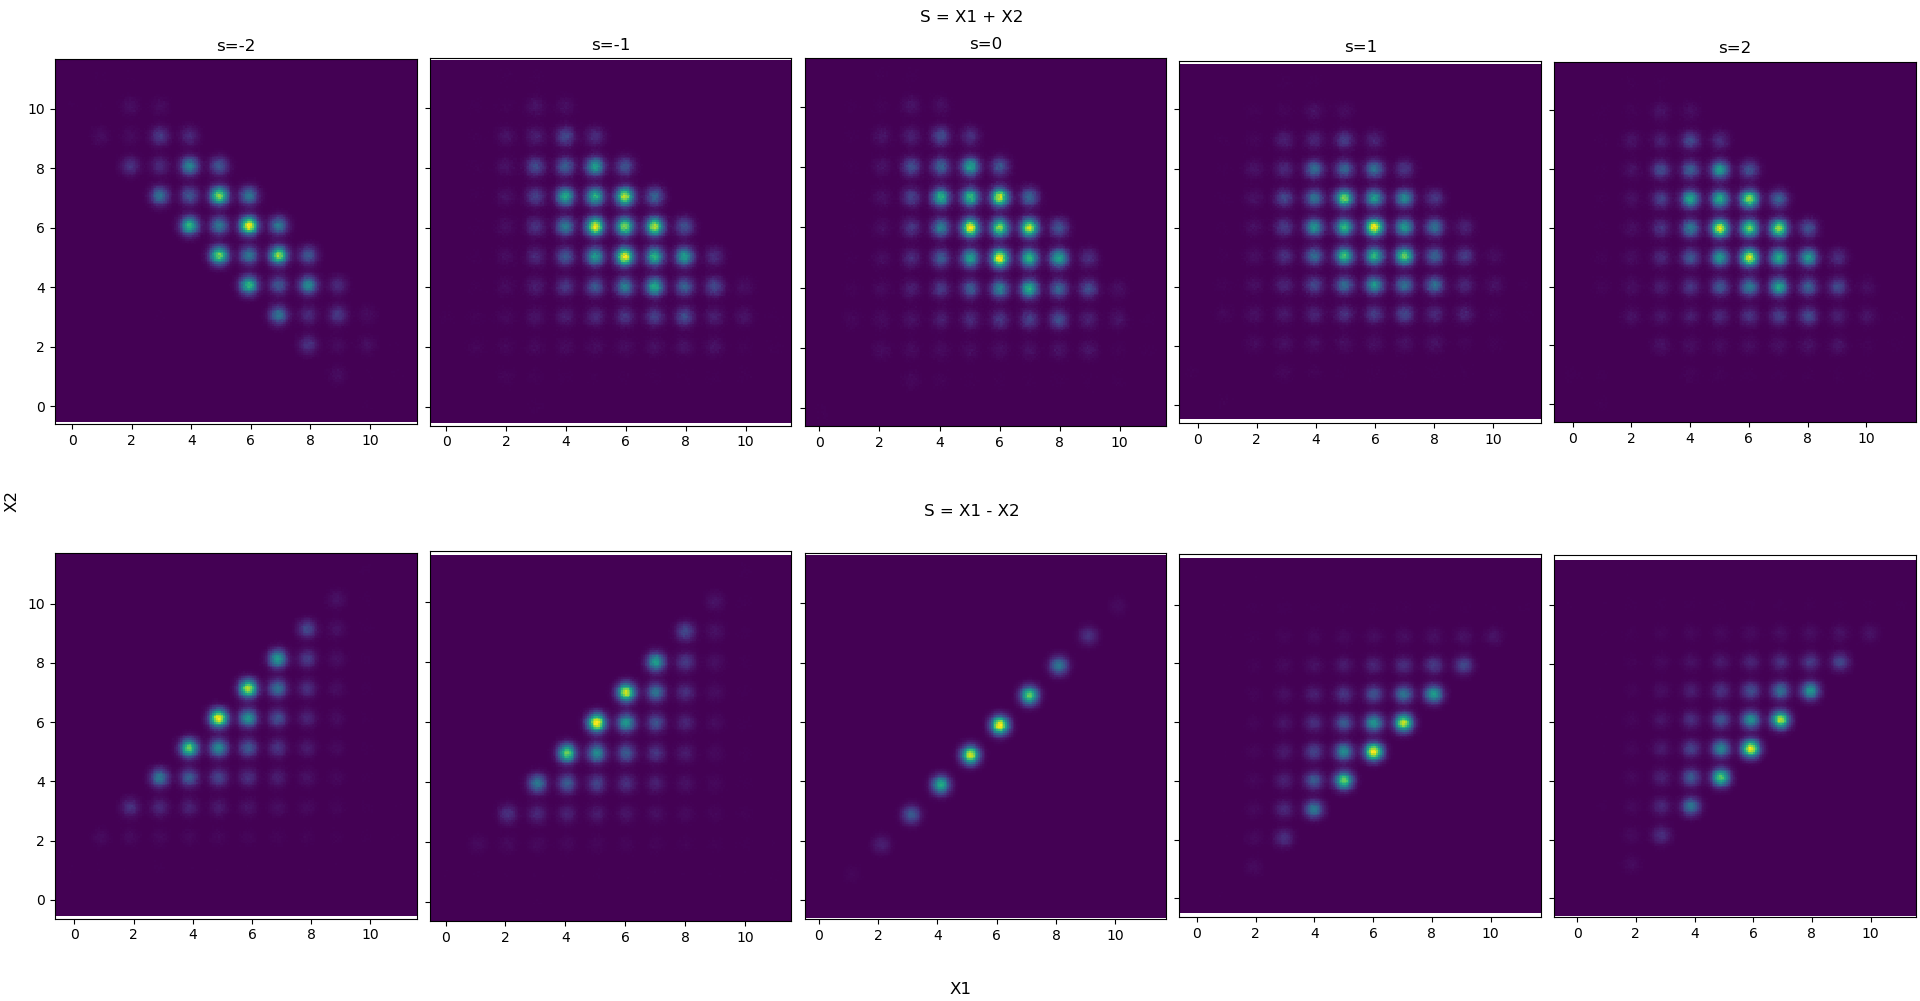
\includegraphics[scale=0.25]{figures/3329_dist_modes.png}
		\caption{2-share leakage distributions over $\mathbb{Z}_Q$.}\label{fig:dist}\vspace*{-0.0cm}
	\end{figure}
	
	\subsection{Quantify observations}
	We next evaluate concretely the information exposed from the leakages of different encoding representations by its MI with the sensitive variable $S$. With $f(li|xi)$ described in Eq.\ref{eq:gl}, we first compute $p(x_i|l_i)$ followed Bayes theorem as in Eq.\ref{eq:f2p}, we, then, obtain $p(s|\bm{l})$ from SASCA. We let $d$ runs from 2 to 6 and $\sigma^2$ runs from $10^{-3}$ to $10^2$, the results are shown in Fig.\ref{fig:mi234}.
	\begin{figure}[h]
		
		\begin{subfigure}{0.5\textwidth}
			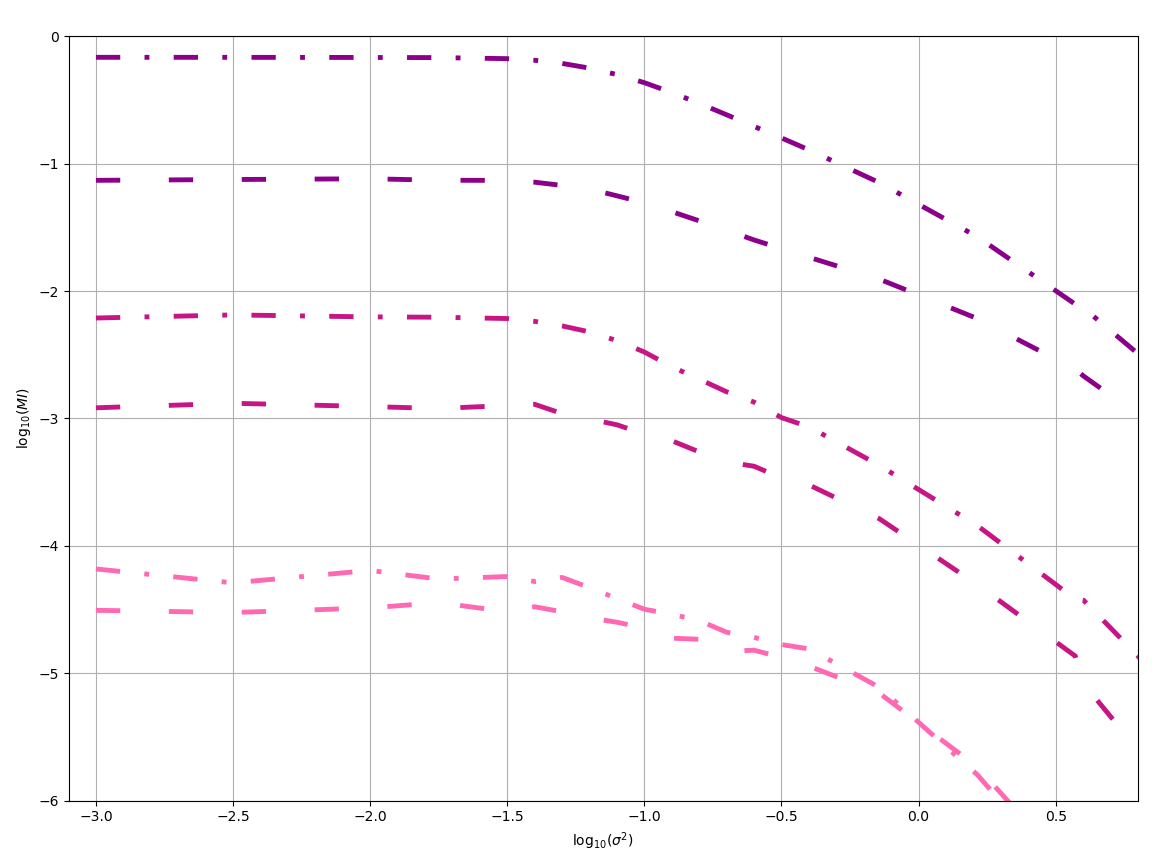
\includegraphics[scale=0.14]{figures/mi_234.png} 
			\caption{MI on simulated data $d$ from  2 to 4 shares, dashed line, dot-dashed lines correspond to $\text{Enc}^{\text{sum}}$, $\text{Enc}^{\text{diff}}$ respectively.}\label{fig:mi234}
		\end{subfigure}
		\begin{subfigure}{0.5\textwidth}
			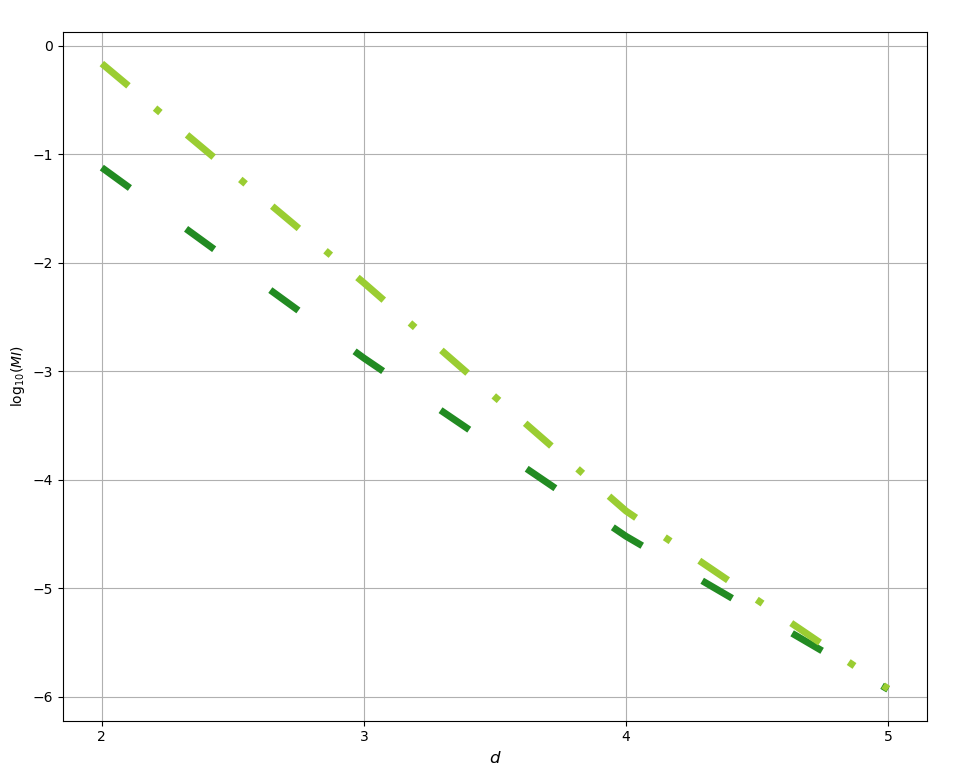
\includegraphics[scale=0.16]{figures/mi_lines_modes.png} 
			\caption{MI on noiseless leakages w.r.t. $d$, dashed line, dot-dashed lines correspond to $\text{Enc}^{\text{sum}}$, $\text{Enc}^{\text{diff}}$ respectively..}\label{fig:milines}
		\end{subfigure}
		\label{fig:image2}
	\end{figure}
	
	There are several noticeable observations from this result:
	\begin{itemize}
		\item First, we confirm once again the noise amplification effect of arithmetic masking in prime-order groups under HW leakage assumption that theoretically hinted in \cite{optimalmask} and experimentally shown in \cite{primemask}. Even when $S$ lies in a small set we still have an exponential increment of security with respect to the number of shares. This trend is stable when noise increases. Additionally, this effect holds in different encoding representations. 
		\item Next, as anticipated, there is a significant gap between two representations, where leakage from $\text{Enc}^{\text{diff}}$ exposes more information about the secret than $\text{Enc}^{\text{sum}}$. This gap is a factor of ten for $d=2$ and seems to decrease when the number of shares increases.
	\end{itemize}
	We want to stress the notable gap between the two representations. There would be no difference to mask $S$ as $\text{Enc}^{\text{diff}}$  or $\text{Enc}^{\text{sum}}$  if $S$ is uniformly distributed over $\mathbb{Z}_Q$ \todo{Show this in A?}. However, when $S$ only takes a few specific values, operations on shares matter. For example, in 2-share case, $s=0$ is exposed totally given $\text{HW}(X_1)$ and $\text{HW}(X_2)$ in  $\text{Enc}^{\text{sum}}$ but there is no such value of $s$ in $\mathcal{S}$ has the same issue if $\text{Enc}^{\text{diff}}$ is used(this could be viewed as an homomorphic attack" as suggested in \cite{optimalmask}).
	
	Additionally, the difference between the two ways of encoding diminishes when the number of shares $d$ increases. We confirm this trend with smaller prime-order group $\mathbb{Z}_{23}$(Fig.\ref{fig:miq23})\todo{Better fig}. We adopt the reduction to random walks as \cite{optimalmask}, and then the length of operation repetition seems to be relevant. For example, in considering $d=4$, we have $S^\text{diff} = X_1 + X_2 + X_3 + X_4$ in $\text{Enc}^{\text{diff}}$  and $S^\text{sum} = -X_1 - X_2 - X_3 + X_4$   in $\text{Enc}^{\text{sum}}$ then intuitively, $Z_1 + Z_2 + Z_3 + Z_4$ is close to uniform than $-Z_1 - Z_2 - Z_3 + Z_4$. By trying two other representations:
	\begin{align*}
		S^1 &= -X_1 + X_2 + X_3 + X_4\\
		S^2 &= -X_1 - X_2 + X_3 + X4,
	\end{align*}
	and compute MI corresponds to each one in the same manner, we obtain results depicted in Fig.\ref{fig:mi_4shares}.
	\begin{figure}[!h]
		\vspace*{-0.0cm}
		\hspace*{0.0cm}\centering 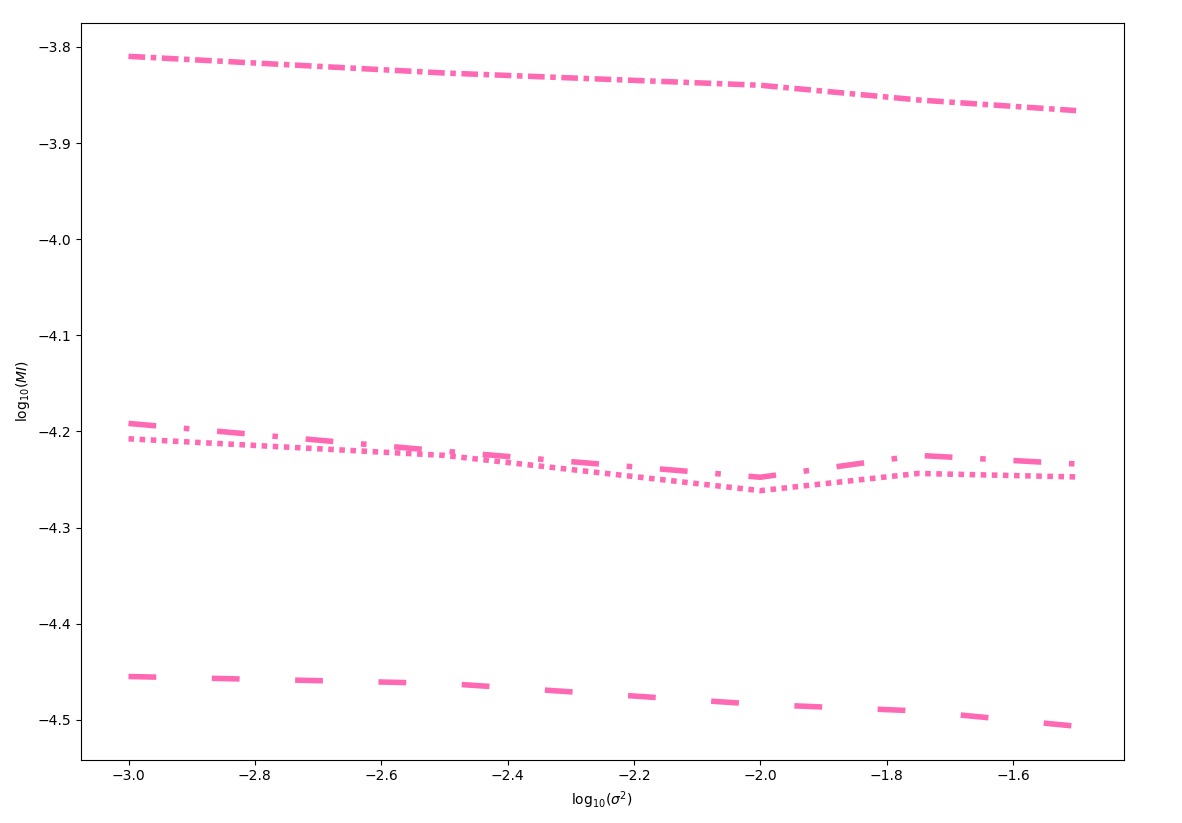
\includegraphics[scale=0.2]{figures/4shares_modes.png}
		\vspace*{0.3cm}
		\caption{MI for four different representations for 4-share encoding.\\ densely dash-dotted, loosely dash-dotted, dotted, dashed are $S^2$, $S^{\text{sum}}$, $S^1$ and $S^{\text{diff}}$ respectively}\label{fig:mi_4shares}\vspace*{-0.0cm}
	\end{figure}
	\todo{Better fig}
	
	It somehow infers the impact of operation repetition, as suspected. Where this length is equal and is 3 in $S^\text{sum}$ and $S^1 $, we gain the same amount of information about $S$ given $\bm{L}$. We have the least in $S^\text{diff}$ where this length is the longest (i.e., 4) and have the most information in $S^2$ where this length is 2.
	
	We emphasize that this interpretation is merely experimental and lacks of concrete theoretical proof. However, we are certain that this trend can be explained in a formal manner.
	\section{Real-world analysis}\label{sec:onm}
	We next put the observations in simulation to test with real measurements.
	
	We note that several available polynomial masking for KYBER \cite{Kmaskimp0},\cite{Kmaskimp1}, \cite{Kmaskimp2} and all polynomial masking schemes for KYBER (especially and for PQC in general) such as \cite{Kmask1} \fxnote[]{more citations} use $\text{Enc}^{\text{diff}}$ for their representation. This is a positive sign as it has been shown in simulation that it allows exponential security with respect to the number of shares $d$ and $\text{Enc}^{\text{diff}}$ provide better security compared to $\text{Enc}^{\text{sum}}$. However, depending on the implementation, the leakage can actually be in the form of $\text{Enc}^{\text{sum}}$. Normally, to mask a coefficient of the secret $s$, the computations follow:
	\begin{enumerate}
		\item Copy $s$ to the last (or the first) share $x_d \leftarrow s$.
		\item Generate a random number $r$ in $\mathbb{Z}_Q$.
		\item Assigning the shares and accumulating them can be done in two ways:
		\begin{itemize}
			\item Assign $x_i \leftarrow r$ and accumulate on the last share $x_d = x_d - r$, or
			\item Assign $x_i \leftarrow Q - r$ and $x_d = x_d + r$.
		\end{itemize}
	\end{enumerate}
	Both ways in step 3 eventually lead to $\text{Enc}^{\text{diff}}$ representation but notice if we have that leakage corresponding to $r$ then the second ways of computing share gives us the leakage corresponding to $\text{Enc}^{\text{sum}}$.
	
	We then use the same implementation such as \cite{Kmaskimp0} but use leakage on $x_i$ and $x_d$ to produce data for $\text{Enc}^{\text{diff}}$ and use leakage on $r$ and $x_d$ to produce data for $\text{Enc}^{\text{sum}}$.
	
	We run our implementations on Arm Cortex-M4 STM32F415 and acquire two million traces for each implementation. We first compute SNR on the data to make sure there is no first-order information of $S$ in the traces and to select relevant PoIs for the next step\footnote{SNR on traces are shown in Fig.\ref{fig:snr2}}. In order to compare between implementations, we again base on IT metric and PI to be more specific.
	
	We proceed with our evaluation in several steps:
	\begin{enumerate}
		\item For each share, we select $n_{\text{PoI}}$ points in the traces that have maximum SNR corresponding to that share. We then have truncated leakage $\bm{L}'_i$ for each share. These shares' leakages are then concatenated to be reduced traces $\bm{L}'$ or kept separately depending on the distinguisher in use.
		\item We then use $\bm{L}'$ or $\bm{L}'_i$ to model $p(s|\bm{l}')$ directly or $p(x_i|\bm{l}'_i)$. In the latter case, we combine $p(x_i|\bm{l}'_i)$ to obtain $p(s|\bm{l}')$ eventually.
		\item PI is estimated using Eq.\ref{eq:pi} on the model given by the previous step.
	\end{enumerate}
	
	We use different distinguishers to model the unknown $p(\cdot|\cdot)$ to inspect the leakages in different assumptions. 
	The distinguishers are:
	\begin{description}
		\item[Plain MLP] We feed MLP the reduced traces $\bm{L}'$ and use it to directly model $p_(s|\bm{l})$ and PI is estimated based on MLP's output. The model $p_(s|\bm{l})$ is estimated without any assumption about the leakage. We make sure that the selected points do not have maximal SNR value w.r.t. the secret to avoid any first-order information of the secret.
		\item[MLP x SASCA] We keep truncated traces for each share $\bm{L}'_i$ separately. Then we use MLP to model $p(x_i|\bm{l}_i)$ for each share. The results then are fed to SASCA to obtain $p(s|\bm{l})$. We restrict the information of the secret only from the leakage of its shares. However, there is no assumption on the shares' leakage.
		\item[LDA x SASCA] Similar process as MLPxSASCA, we used truncated traces $\bm{L}'_i$  to build the model for $p(x_i|\bm{l}_i)$ separately using LDA. In LDA, the truncated traces  $\bm{L}'_i$  are projected to a subspace of dimension $n_{\text{LDA}}$, then GMT is applied as described in Sec.\ref{ssec:lda} to obtain  $p(x_i|\bm{l}_i)$. Finally, $p(s|\bm{l})$ is estimated using SASCA. In this setting, shares' leakages are assumed to be multivariate Gaussian distributed and satisfy homoscedasticity.
	\end{description}
	\todo{Optimal  $n_{\text{PoI}}$ , optimal $n_{\text{LDA}}$}
	We compare convergence rates among distinguishers by computing PI correspondingly to the increasing number of profiling traces $N_p$. The results is shown in Fig.\ref{fig:pi}.\todo{Complete this fig}
	\begin{figure}[h]
		\vspace*{-0.0cm}
		\hspace*{0.0cm}\centering 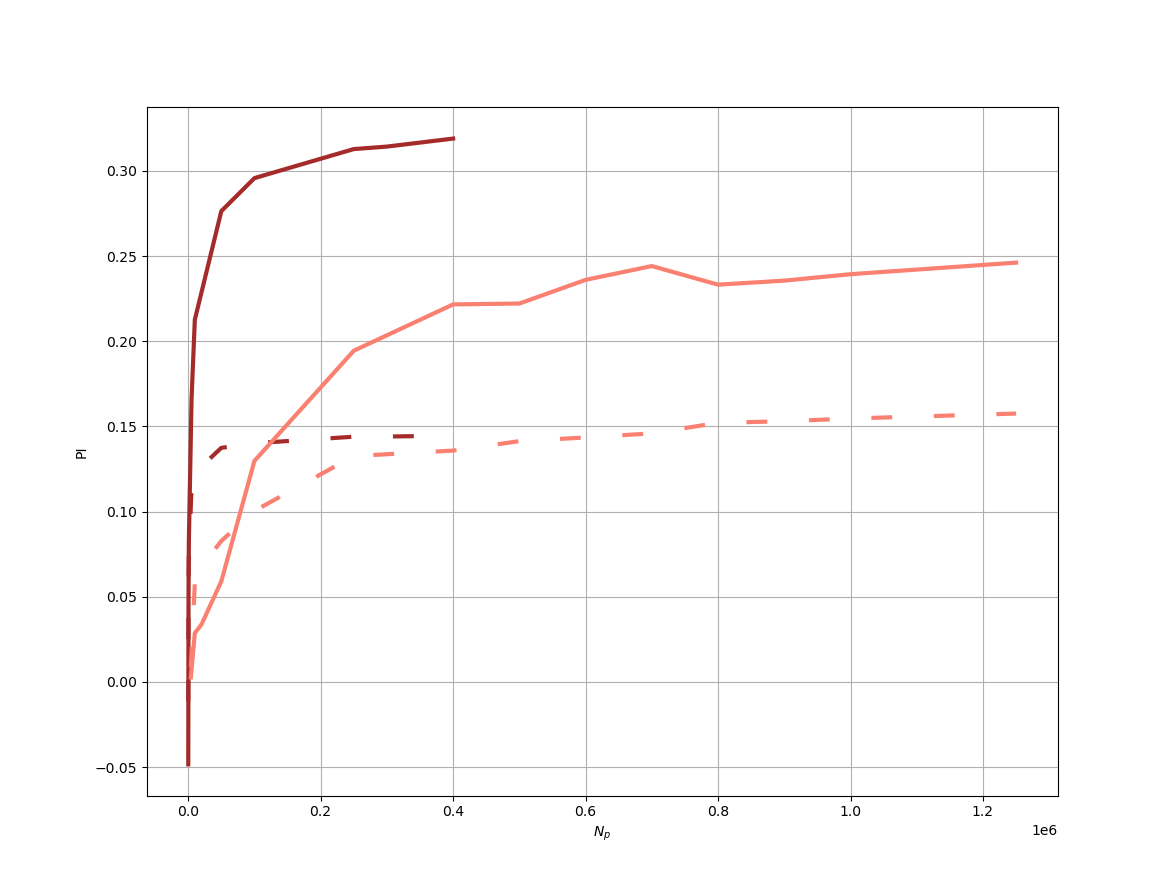
\includegraphics[scale=0.3]{figures/pi_mlps.png}
		\vspace*{0.3cm}
		\caption{PI of different distinguishers. Brown and salmon curves correspond to Plain MLP and MLPxSASCA, solid and dashed curves correspond to $\text{Enc}^{\text{diff}}$ and $\text{Enc}^{\text{sum}}$  respectively.}
		\label{fig:pi}
	\end{figure}
	\section{Conclusion}
	\appendix
	\section{Supplementary}
	\begin{figure}
		\centering
		\begin{subfigure}{1\linewidth}
			\centering
			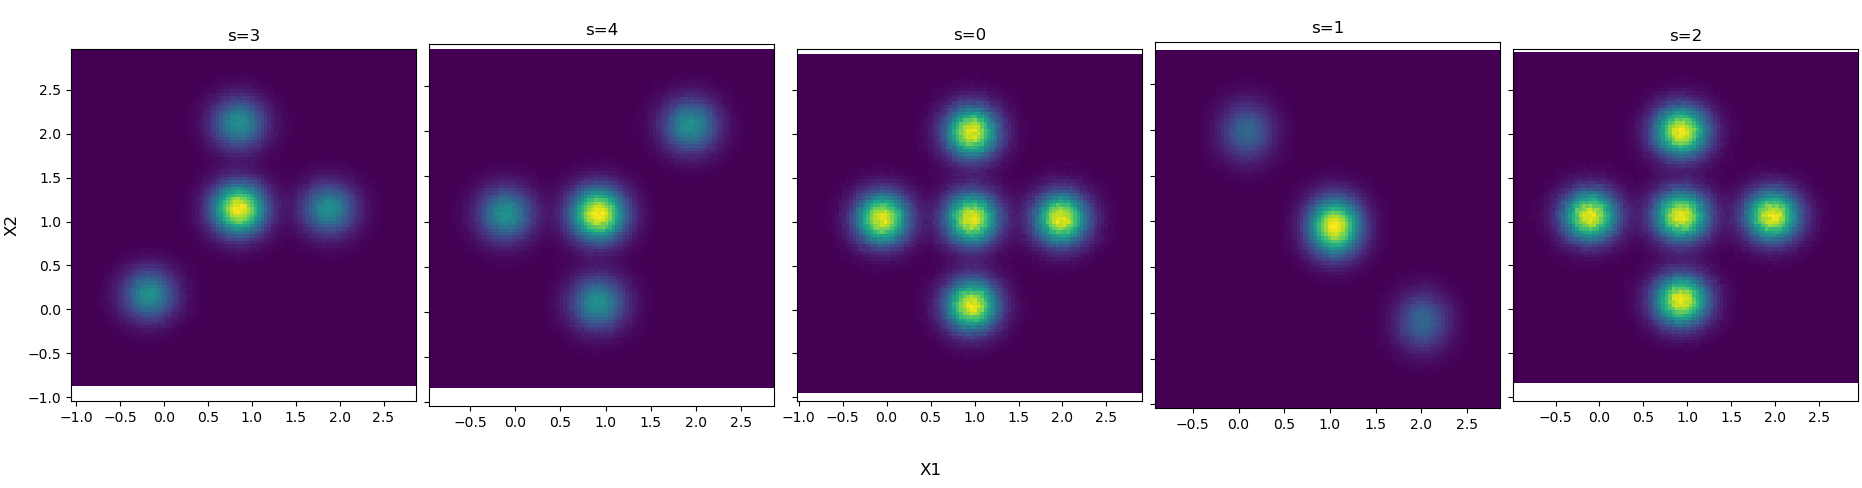
\includegraphics[scale=0.2]{figures/5_dist_sum.png}
		\end{subfigure} %
		
		\hfill
		
		\begin{subfigure}{1\linewidth}
			%\centering
			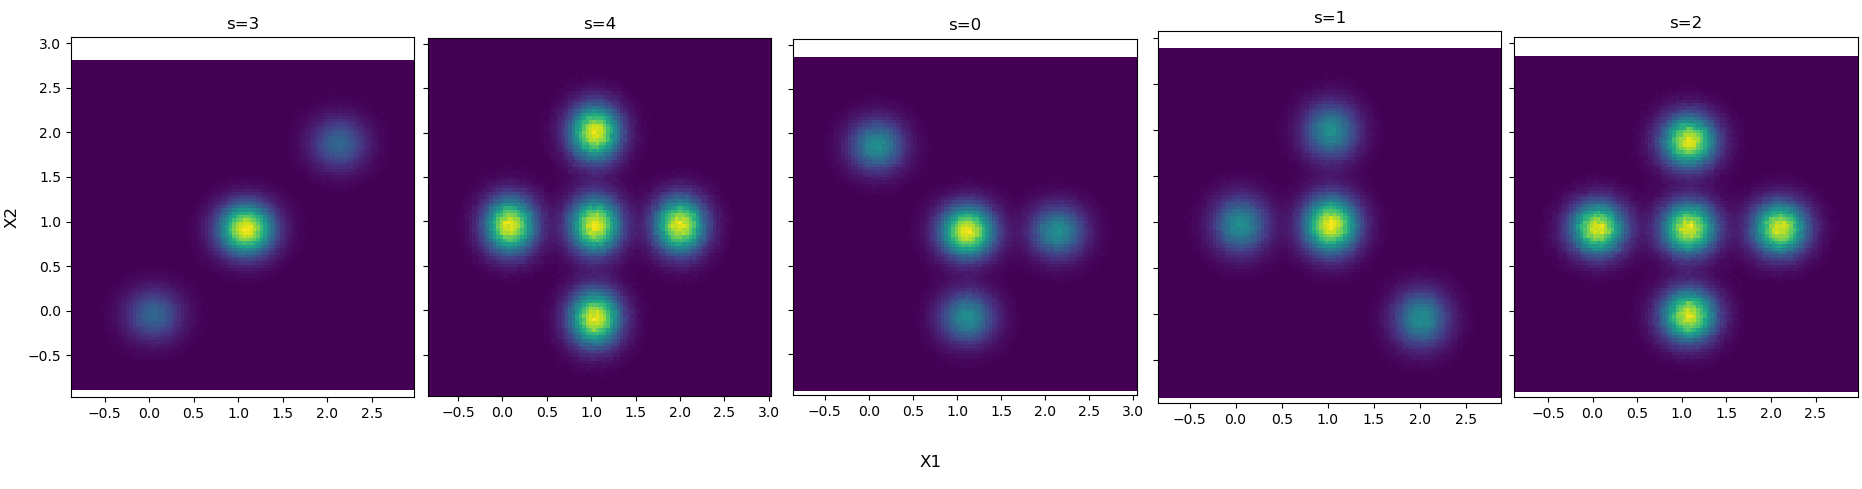
\includegraphics[scale=0.2]{figures/5_dist_diff.png}
		\end{subfigure}
		\caption{Leakages distribution for uniform secret over $\mathbb{Z}_5$. Top and bottom figure is corresponding to  $\text{Enc}^{\text{sum}}$ and  $\text{Enc}^{\text{diff}}$ respectively}
		\label{fig:dist5}
	\end{figure}
	
	\begin{figure}
		\centering
		\begin{subfigure}{1\linewidth}
			\centering
			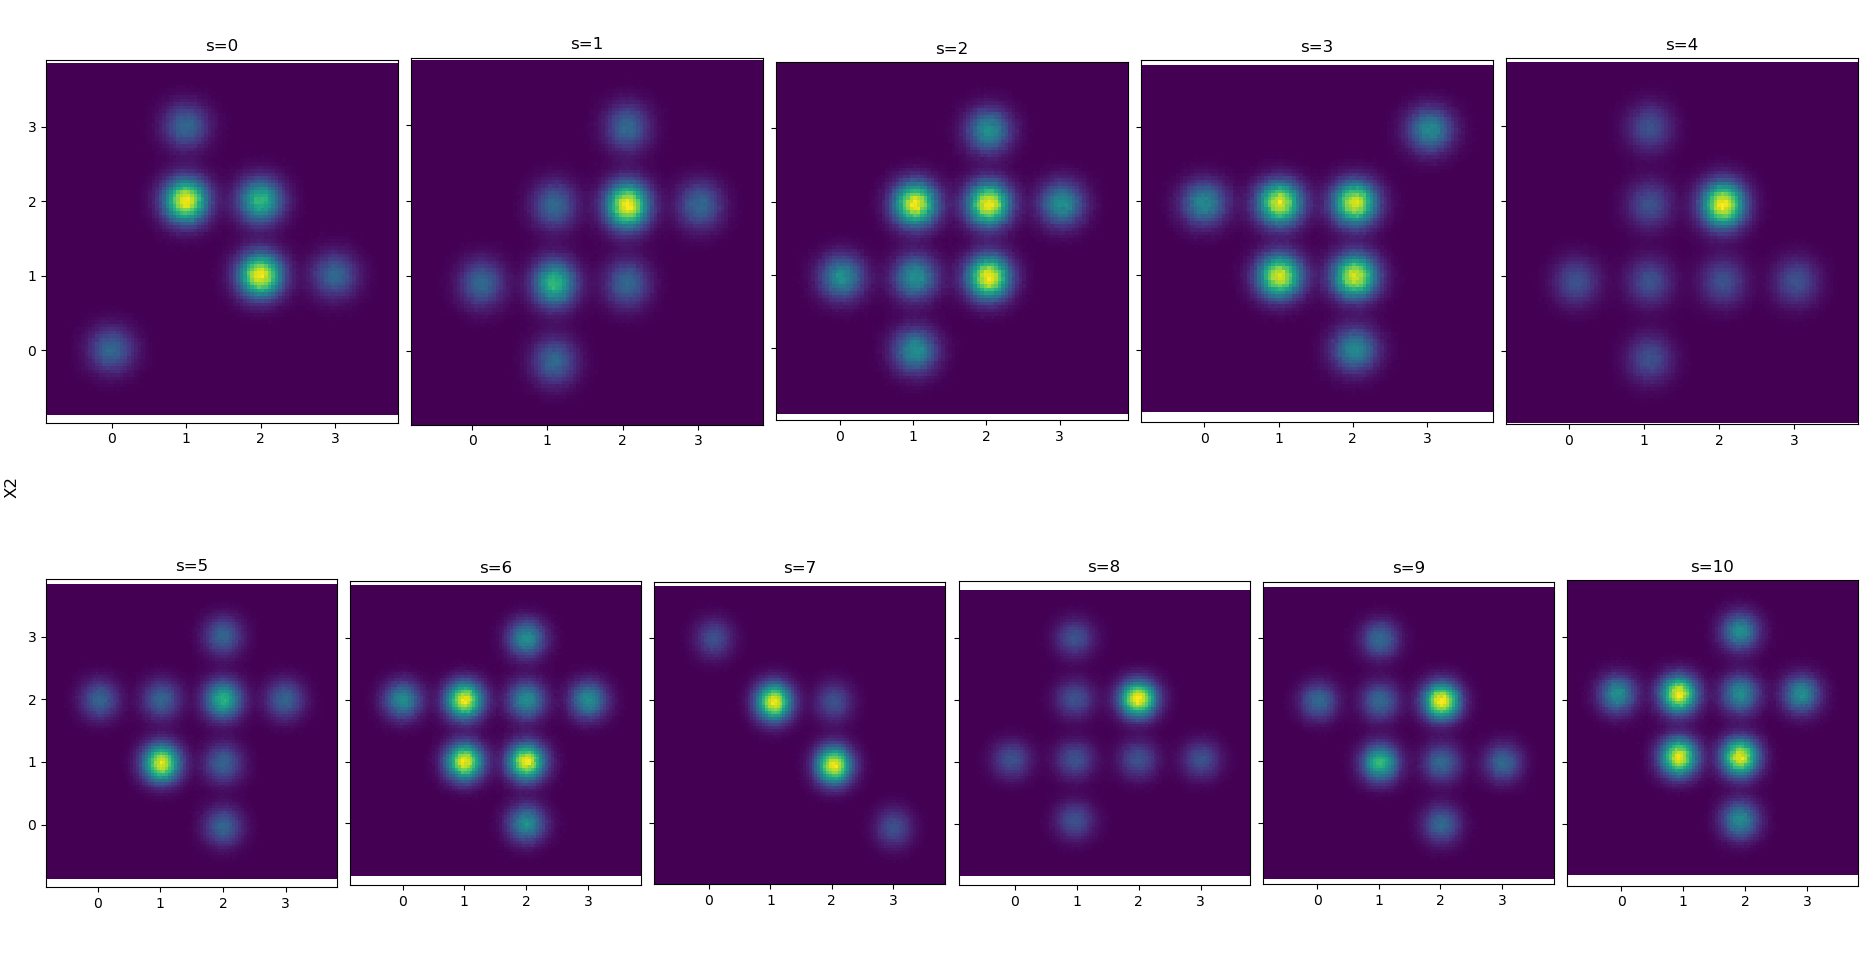
\includegraphics[scale=0.25]{figures/11_dist_sum.png}
			\caption{Leakages distribution of $\text{Enc}^{\text{sum}}$ }
			\label{fig:dist11_sum}
		\end{subfigure} %
		
		\hfill
		
		\begin{subfigure}{1\linewidth}
			%\centering
			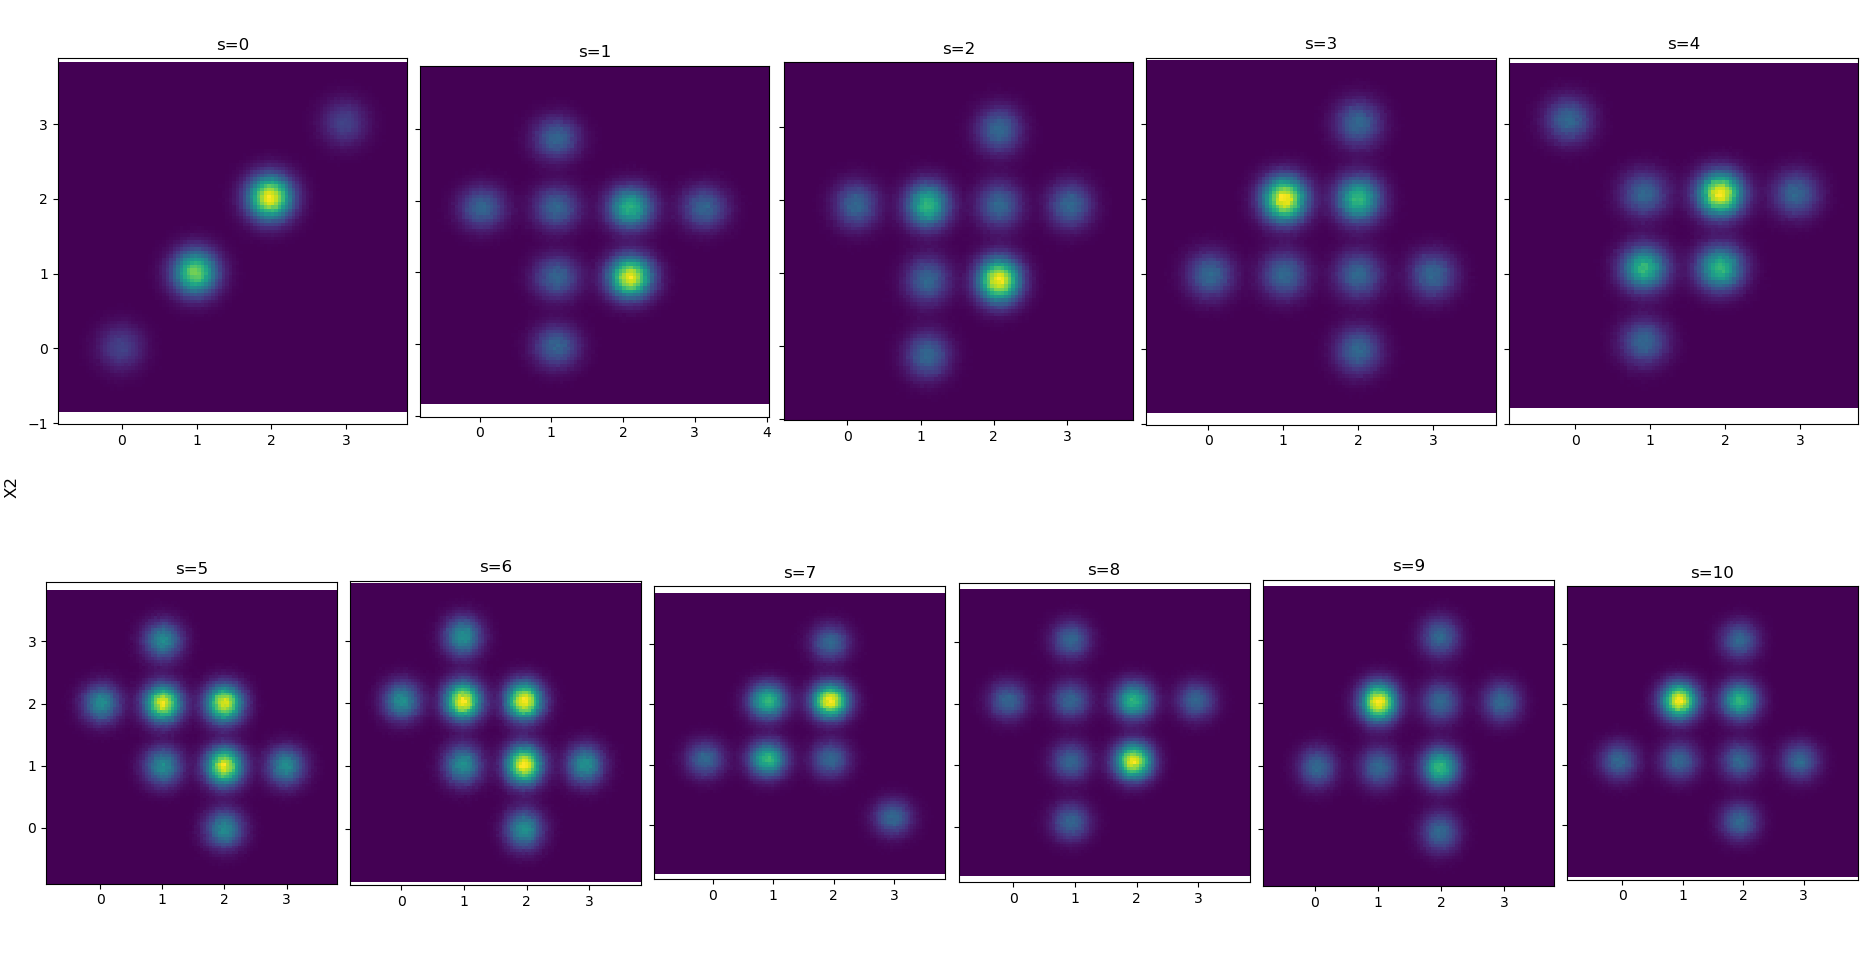
\includegraphics[scale=0.25]{figures/11_dist_diff.png}
			\caption{Leakages distribution of $\text{Enc}^{\text{diff}}$ }
			\label{fig:dist11_diff}
		\end{subfigure}
		\caption{Leakages distribution for uniform secret over $\mathbb{Z}_{11}$, Fig.\ref{fig:dist11_sum} , Fig.\ref{fig:dist11_diff} corresponds to $\text{Enc}^{\text{sum}}$, $\text{Enc}^{\text{diff}}$ respectively.}
		\label{fig:dist11}
	\end{figure}
	
	
	\begin{figure}
		\vspace*{-0.0cm}
		\hspace*{0.0cm}\centering 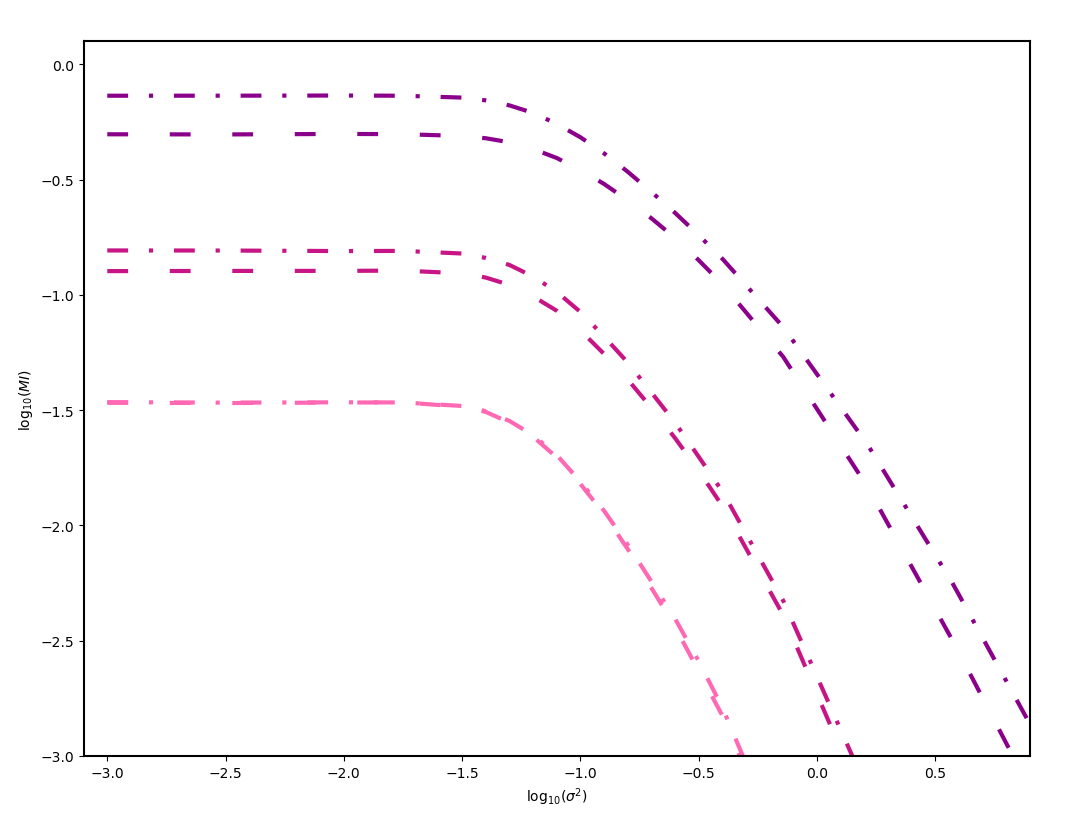
\includegraphics[width=12.0cm]{figures/MI_23_234.png}
		\vspace*{0.3cm}
		\caption{SNR on traces, top figures correspond to $\text{Enc}^{\text{sum}}$, bottom figures correspond to $\text{Enc}^{\text{diff}}$, left figures are SNR on shares where blue and orange line correspond to the first and second share respectively, right figures are SNR on secret.}\label{fig:miq23}\vspace*{-0.0cm}
	\end{figure}
	\begin{figure}
		\vspace*{-0.0cm}
		\hspace*{0.0cm}\centering 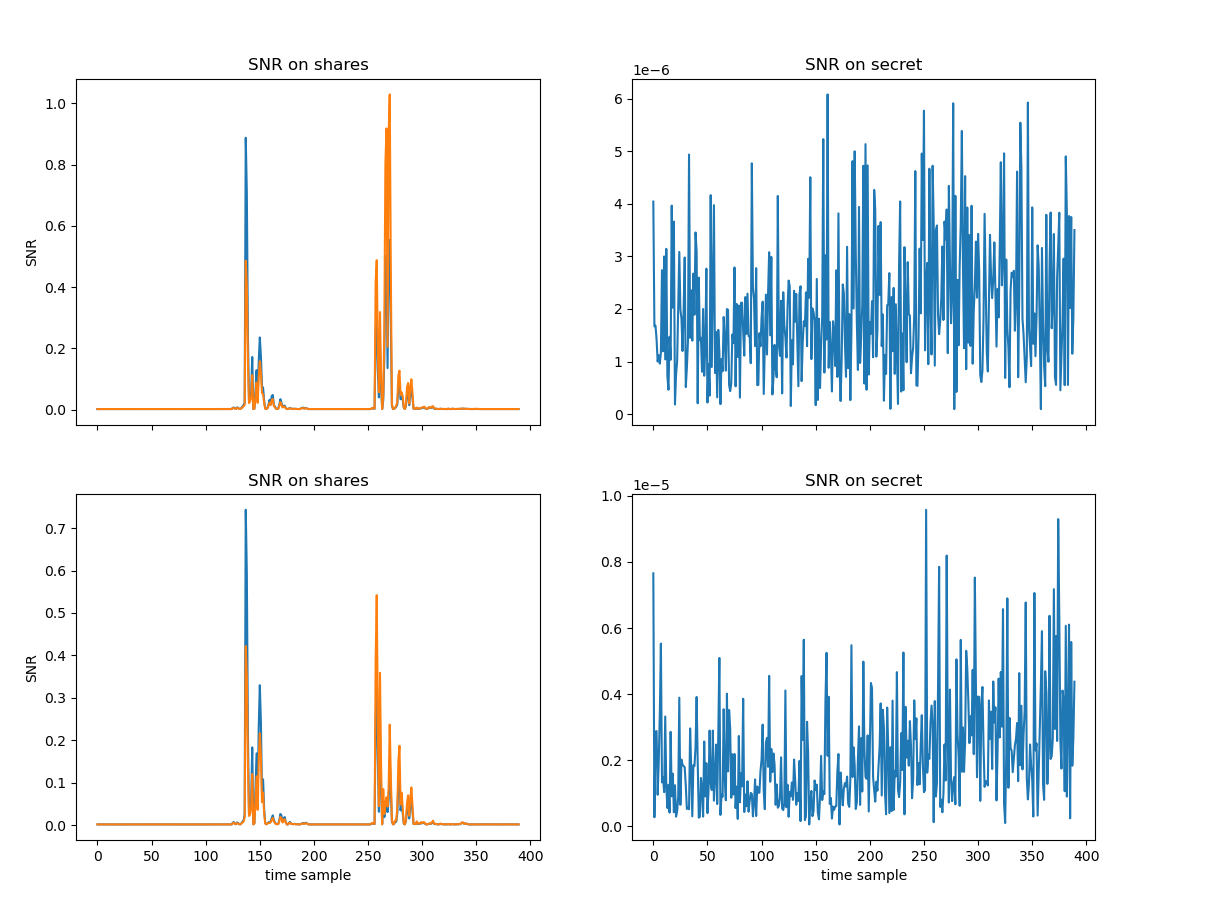
\includegraphics[width=12.0cm]{figures/snr_2shares.png}
		\vspace*{0.3cm}
		\caption{SNR on traces, top figures correspond to $\text{Enc}^{\text{sum}}$, bottom figures correspond to $\text{Enc}^{\text{diff}}$, left figures are SNR on shares where blue and orange line correspond to the first and second share respectively, right figures are SNR on secret.}\label{fig:snr2}\vspace*{-0.0cm}
	\end{figure}
	\bibliographystyle{alpha}
	\bibliography{refs}
	
\end{document}
